\chapter{Baze de date}

Am identificat în literatura de specialitate mai multe lucrări științifice care abordează diferite aspecte ale jocurilor de tenis de masă, printre care TTNet\cite{Voeikov_2020_CVPR_Workshops} realizată de institutul OSAI, care introduce o metodă de analiză și o bază de date publică dedicată tenisului de masă. Ne propunem să realizăm conversia celor două baze de date și să comparăm rezultatele, astfel testând capacitatea sistemului nostru de a generaliza în contexte noi. 


\section{Baza de date FMI-TT}  

\begin{figure}[H]
    \centering
    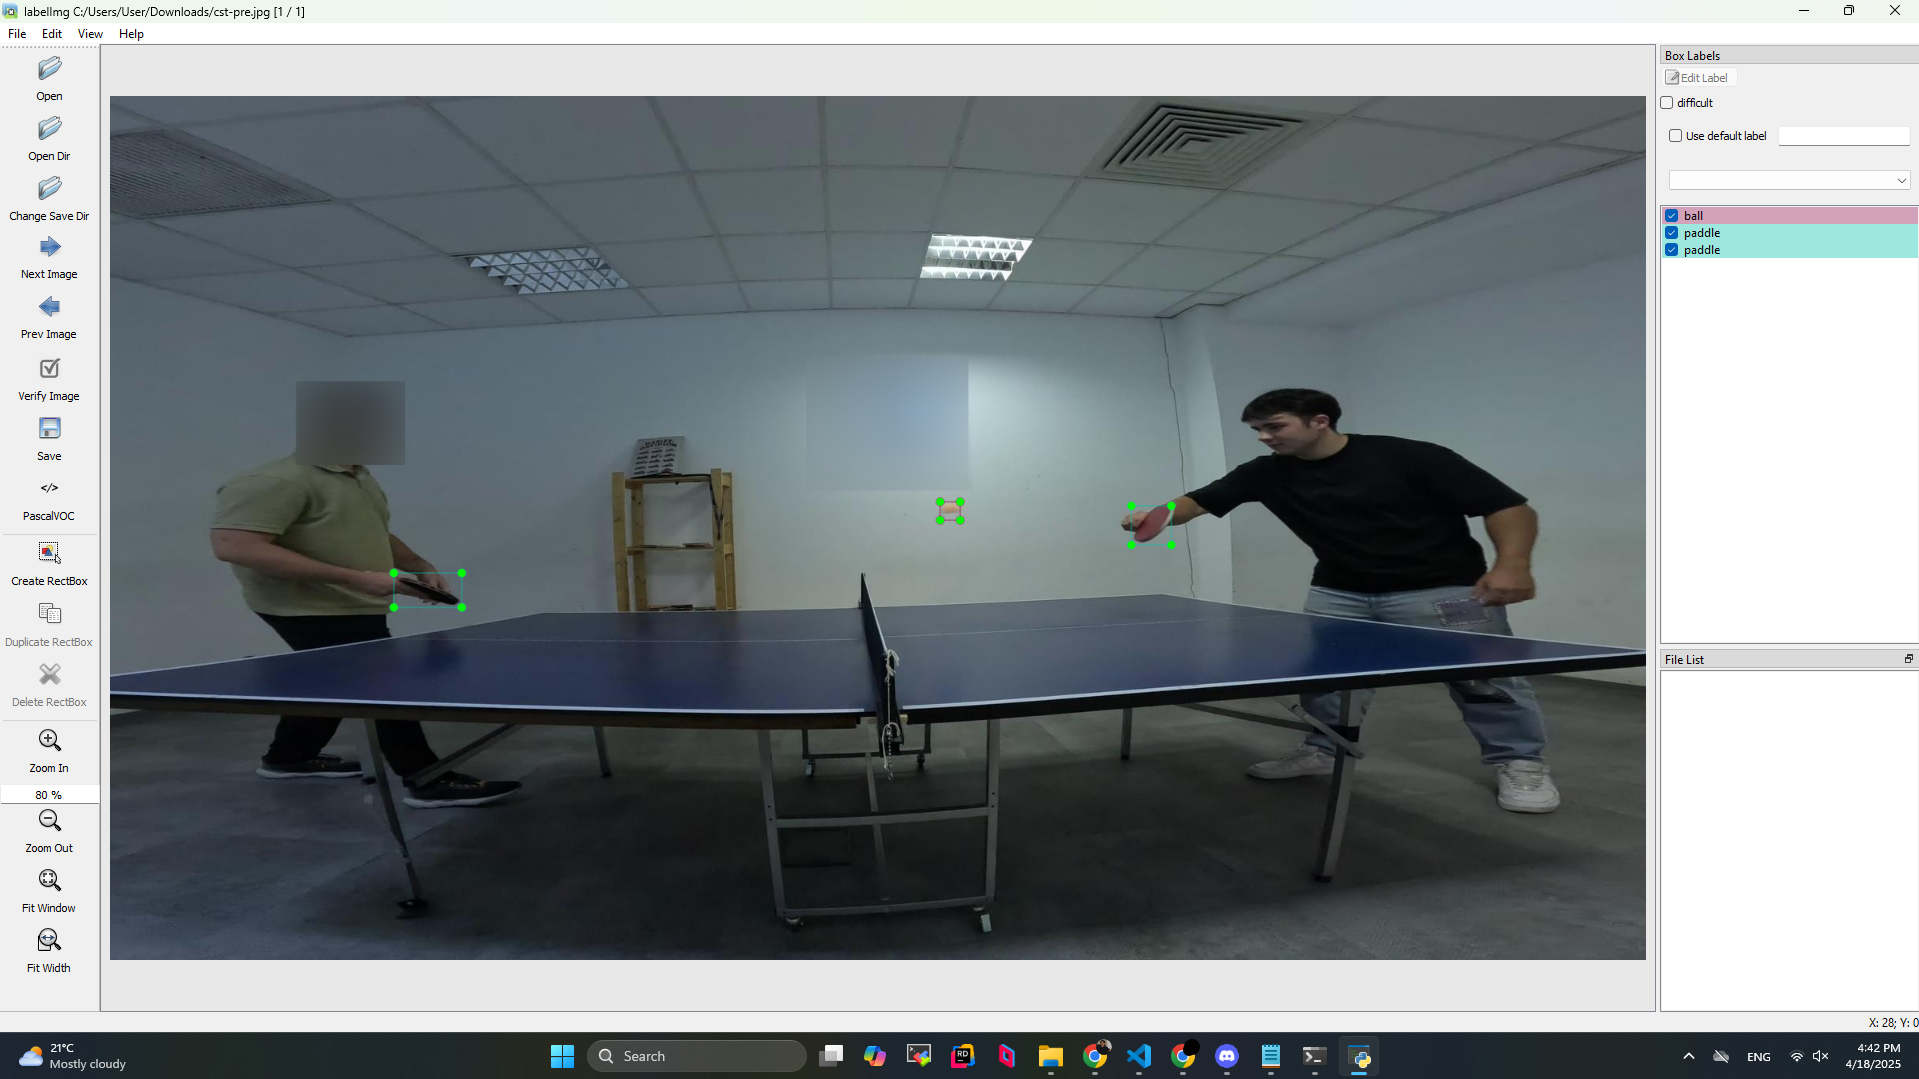
\includegraphics[width=0.8\linewidth]{images/labelimg.png}
    \caption{Adnotarea imaginilor cu labelImg.}
    \label{fig:labeimg-ex}
\end{figure}

Baza de date constă în videoclipuri filmate atât în interior, în lumină artificială, cât și în exterior, în lumină naturală. Evenimentele sunt înregistrate cu echipamente video uzuale, precum telefoane mobile sau camere de filmat, iar ulterior sunt adnotate manual, utilizând \texttt{labelImg}\cite{labelimg}, care produce un fișier \texttt{.txt} cu fereastra de încadrare a fiecărui obiect, un exemplu poate fi regăsit în Figura \ref{fig:labeimg-ex}. De asemenea, baza de date include secvențe de videoclipuri filmate simultan cu două aparate de înregistrare similare. Exemple din baza de date FMI-TT pot fi regăsite în Figura~\ref{fig:cst-pre} și Figura~\ref{fig:double-pre}.

Pentru fiecare obiect, se utilizează formatul \texttt{YOLO}\cite{glenn_jocher_2020_4154370}, în care fiecare linie din fișierul de adnotări conține: numărul clasei, coordonatele centrului \((x, y)\) ale ferestrei de încadrare, lățimea și înălțimea, toate normalizate în funcție de dimensiunea imaginii. Obiectele adnotate sunt: mingea și paletele de tenis de masă.


Baza de date este împărțită în \textbf{1750} de imagini pentru antrenare și \textbf{250} de imagini pentru testare.

\section{Baza de date TTNet}  

Baza de date este constituită din meciuri de tenis de masă filmate în interior, cu echipamente specializate, iar un exemplu poate fi regăsit în Figura~\ref{fig:osai-pre}. Adnotarea cadrelor constă în:

\begin{itemize}
    \item Segmentarea semantică, pentru fiecare cadru, a obiectelor prezente în scenă, un exemplu poate fi regăsit în Figura~\ref{fig:osai-segmented}. În acest proces:
    \begin{itemize}
        \item Jucătorii sunt marcați cu \textbf{verde};
        \item Masa de tenis este marcată cu \textbf{roșu};
        \item Tabela scorurilor este marcată cu \textbf{albastru}.
    \end{itemize}
    
    \item Un fișier JSON care indică poziția \((x, y)\) pentru centrul mingii de tenis de masă.

    \item Un fișier JSON ce conține evenimentele prezente în acel cadru, mai exact:
    \begin{enumerate}
        \item \texttt{bounce} – contactul mingii cu masa;
        \item \texttt{net} – contactul mingii cu fileul;
        \item \texttt{empty event} – eveniment utilizat astfel încât modelul să nu facă predicții doar între \texttt{bounce} și \texttt{net}.
    \end{enumerate}
\end{itemize}

Baza de date include \textbf{39.162} de imagini pentru antrenare, \textbf{9.513} de imagini pentru validare și \textbf{7.332} de exemple pentru testare.

\begin{figure}[H]
    \centering
    \begin{subfigure}[b]{0.48\linewidth}
        \centering
        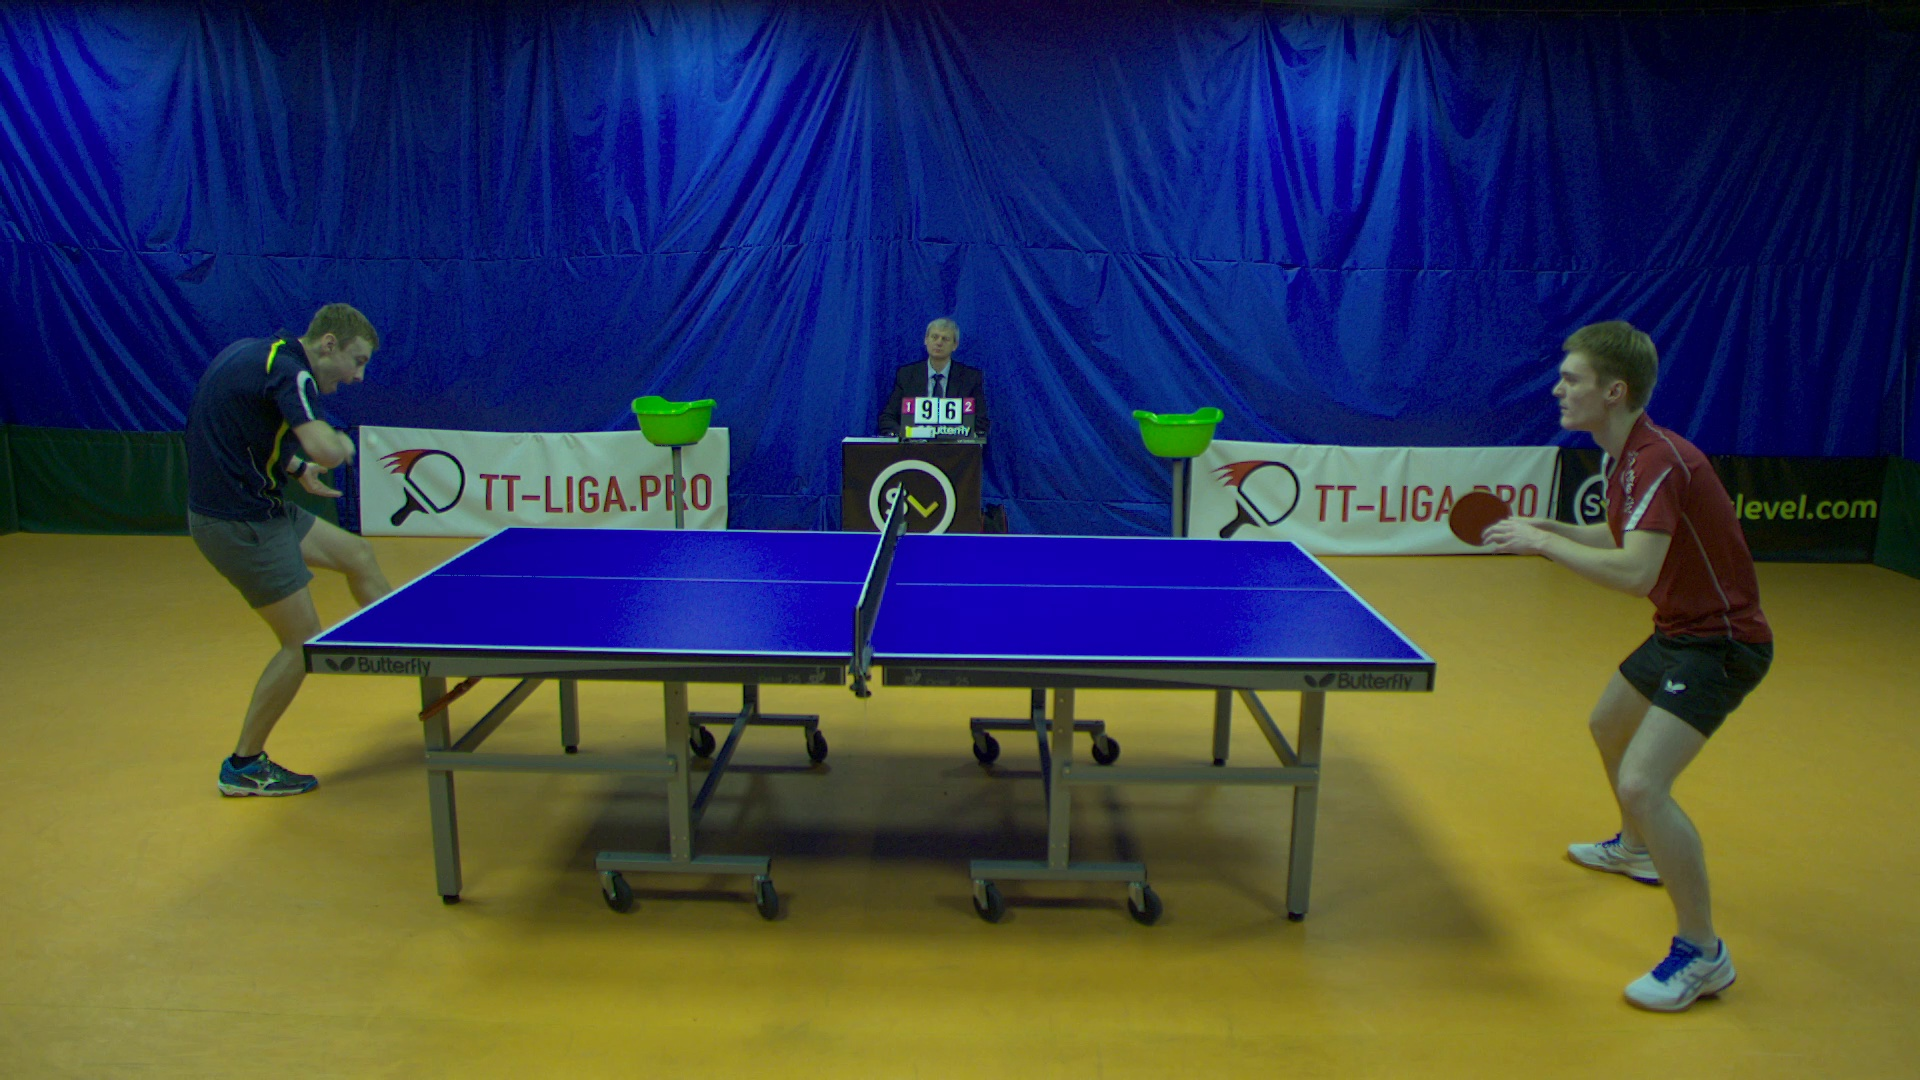
\includegraphics[width=\linewidth]{images/osai-pre-seg.jpg}
        \caption{Cadru neprocesat.}
        \label{fig:original}
    \end{subfigure}
    \hfill
    \begin{subfigure}[b]{0.48\linewidth}
        \centering
        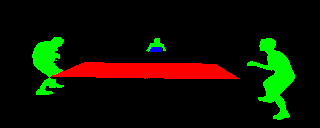
\includegraphics[width=\linewidth]{images/osai-segmented.png}
        \caption{Segmentarea semantică a cadrului.}
        \label{fig:osai-segmented}
    \end{subfigure}

    \caption{Compararea imaginii originale și a segmentării semantice.}
    \label{fig:comparatie-segmentare}
\end{figure}

\section{Postprocesarea datelor}

Ne propunem să adaptăm baza de date FMI-TT la structura bazei de date TTNet și reciproc, pentru a permite rularea ambelor metode și obținerea unei verificări încrucișate a rezultatelor. După implementarea algoritmului și conversia datelor, vom antrena ambele metode pe propriile baze de date. Ulterior, vom relua procesul de antrenare cu o rată de învățare mai scăzută asupra bazei de date postprocesată, astfel încât să nu influențăm major ponderile deja învățate, dar totuși să acomodăm scenarii noi.

\subsection{Postprocesarea bazei de date FMI-TT}
\label{subsec:personal-dataset}

\subsubsection{Adnotarea mingii de tenis de masă}
Întrucât baza de date TTNet necesită doar coordonatele centrului mingii, vom adapta un script care să transforme fișierul \texttt{.txt} în format JSON. Astfel, pentru fiecare adnotare din format YOLO, vom păstra doar centrul mingii, ignorând înălțimea și lățimea acesteia.

\subsubsection{Adnotarea evenimentelor}
\label{subsec:event-adnotation}
Evenimentele adnotate în jocurile de tenis de masă sunt relativ rare, astfel încât intervenția manuală este posibilă. În acest scop, vom utiliza un script scris în Python care folosește biblioteca Tkinter\cite{tkinter} pentru a genera o interfață grafică. Aceasta oferă comenzi rapide de la tastatură ce ne permit să parcurgem imaginile dintr-un director și să le adnotăm eficient, comenzile sunt:
\begin{itemize}
    \item \texttt{N} – trecerea la imaginea următoare;
    \item \texttt{P} – revenirea la imaginea anterioară;
    \item \texttt{E} – marcarea unui eveniment;
    \item \texttt{1}, \texttt{2}, \texttt{3} – alegerea tipului de eveniment \textit{bounce}, \textit{net}, \textit{empty event}.
\end{itemize}

\subsubsection{Adnotarea mesei de tenis și a jucătorilor}
\label{subsec:table-notation}
\begin{figure}[H]
        \centering
        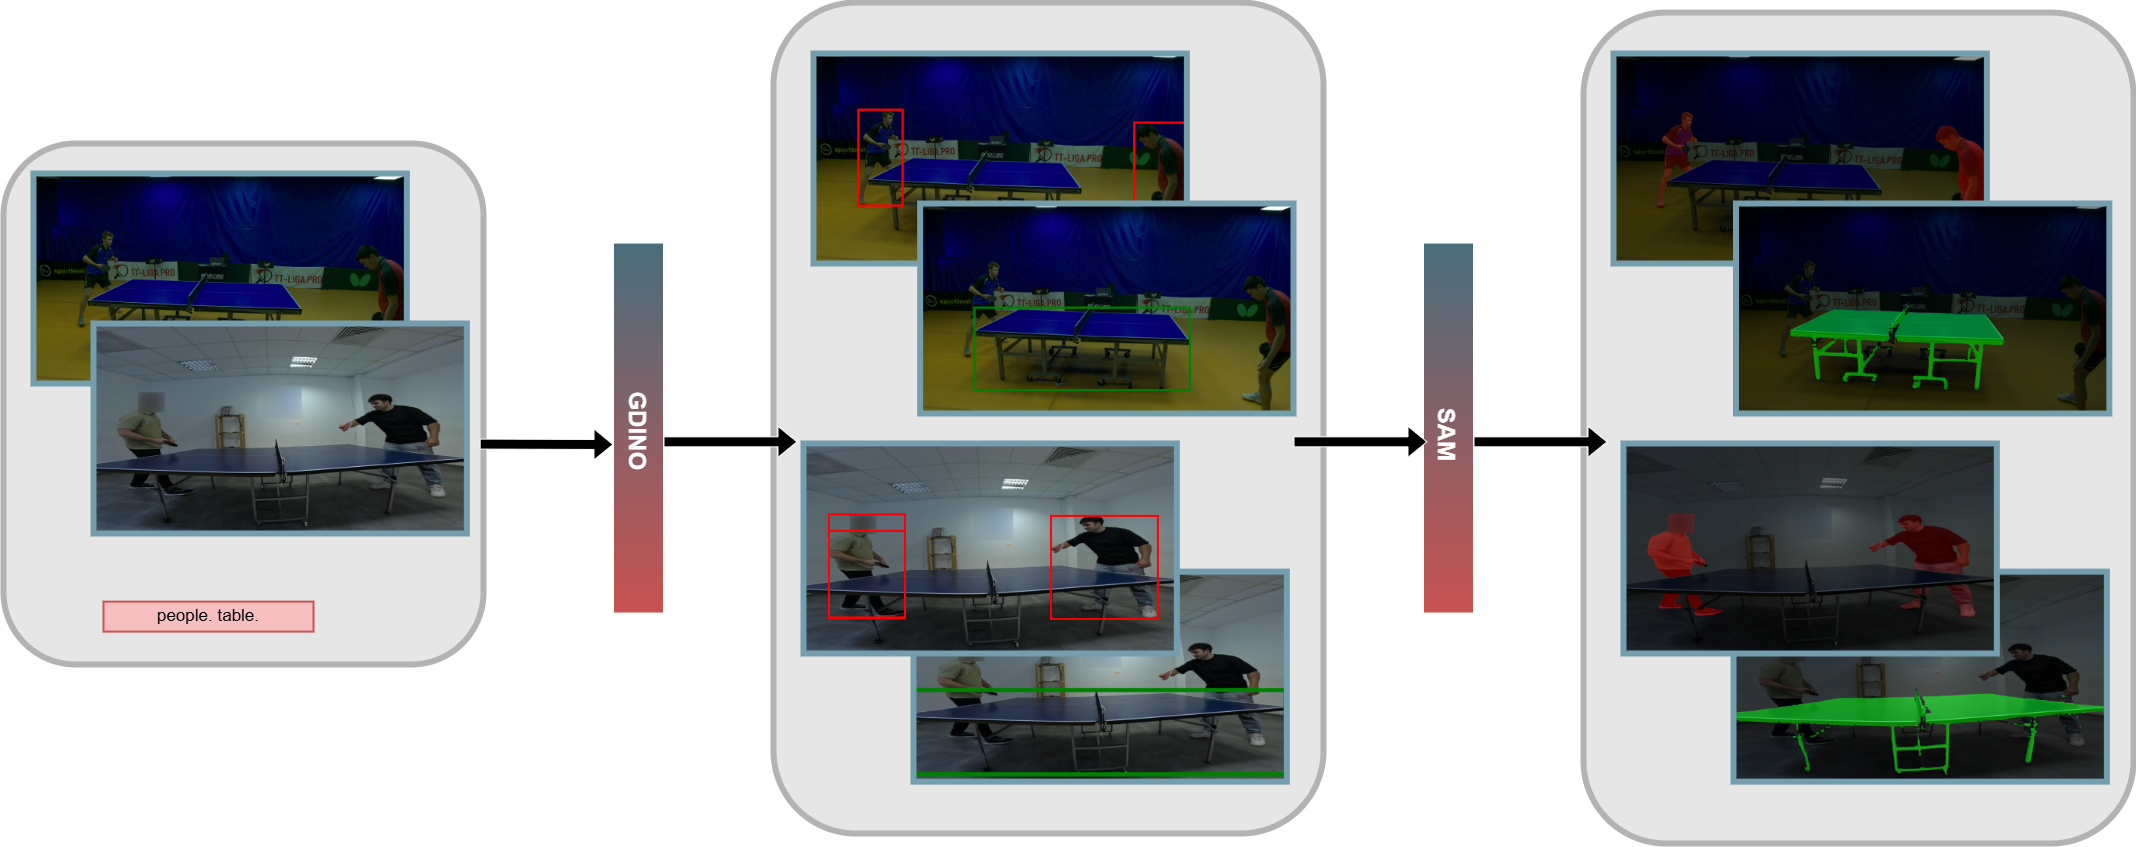
\includegraphics[width=1\linewidth]{images/GSAM3.png}
        \caption{Arhitectura \textbf{GDINO} și \textbf{SAM}.}
        \label{fig:enter-label}
    \end{figure}

În cadrul segmentării semantice a jucătorilor și a mesei, vom implementa o soluție mai avansată, întrucât aceste elemente sunt reprezentate la nivel de pixel, iar încadrarea lor manuală într-o mască ar fi consumatoare de timp și predispusă la erori umane.

Prin urmare, vom opta pentru un sistem de adnotare automată, utilizând următoarele arhitecturi neuronale: \textbf{GDINO}\cite{liu2023grounding}, care returnează ferestre de încadrare însoțite de scor pentru \textit{prompt-urile} text, și \textbf{SAM}\cite{kirillov2023segany}, care returnează 3 măști de segmentare semantică pentru fiecare fereastră de încadrare. 

În Algoritmul~\ref{alg:gsam}, pentru fiecare imagine extragem cu \textbf{GDINO} setul de ferestre de încadrare și scoruri, $\mathcal{B}_{t,p}=\{(b_i,s_i)\}_{i=1}^{n}$. Eliminăm ferestrele cu scor mai mic decât 0.5, iar apoi aplicăm \textbf{SAM} pentru fiecare fereastră rămasă, obținând multiple măști de segmentare pe care le unificăm pentru a obține masca finală a imaginii. Un exemplu de rezultat apare în Figura~\ref{fig:comparatie-segmentare}.

\begin{figure}[H]
    \centering
    \begin{subfigure}[b]{0.48\linewidth}
        \centering
        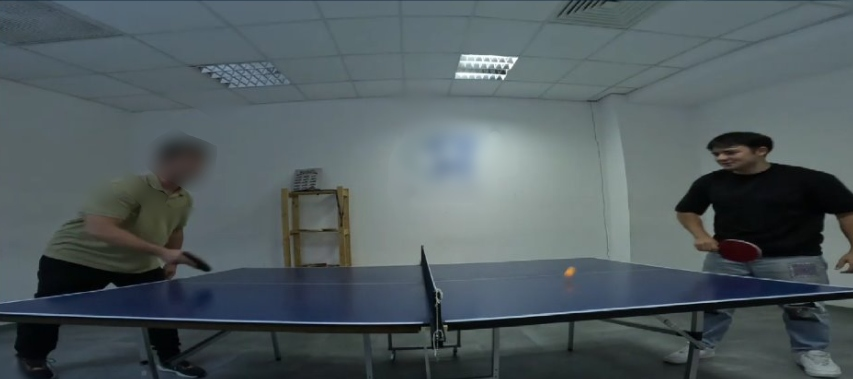
\includegraphics[width=\linewidth]{images/cst-before-sam.jpg}
        \caption{Cadru neprocesat.}
        \label{fig:original}
    \end{subfigure}
    \hfill
    \begin{subfigure}[b]{0.48\linewidth}
        \centering
        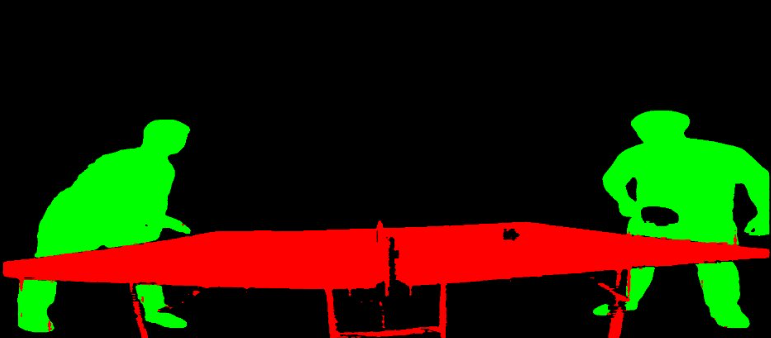
\includegraphics[width=\linewidth]{images/cst-after-sam.png}
        \caption{Segmentarea semantică a cadrului.}
        \label{fig:segmented}
    \end{subfigure}

    \caption{Compararea imaginii originale cu segmentarea semantică.}
    \label{fig:comparatie-segmentare}
\end{figure}

\begin{algorithm}[H]
\caption{Segmentarea automată a jucătorilor și mesei de tenis.}
\label{alg:gsam}
\begin{algorithmic}[1]
\Require Secvență de imagini: $\{I_t\}_{t=1}^{T}$
\Ensure Secvență de imagini segmentate semantic: $\hat{\{I_t\}}_{t=1}^{T}$
  \For{$t \gets 1$ \textbf{la} $T$}
    \State $M_{t,\textit{people}} \gets \emptyset$
    \State $M_{t,\textit{table}}  \gets \emptyset$
    \ForAll{categorie $p \in \{\textit{"people"},\,\textit{"table"}\}$}
      \State $\mathcal{B}_{t,p} \gets \mathrm{GDINO}(I_t, p)$
      \ForAll{$(b, s) \in \mathcal{B}_{t,p}$}
        \If{$s > 0.5$}
            \State $M_{t,p} \gets M_{t,p} \;\cup\; \mathrm{SAM}(I_t, b)$ 
        \EndIf
      \EndFor
    \EndFor
    \State $\hat I_t \gets \mathrm{color}(M_{t,\textit{people}},\text{verde})\;\cup\;\mathrm{color}(M_{t,\textit{table}},\text{roșu})$
\EndFor
  
\end{algorithmic}
\end{algorithm}

Această prelucrare se realizează pe baza unui director de intrare și unul de ieșire, astfel încât am putut transforma cele 2000 de imagini din FMI-TT.

\subsection{Postprocesarea bazei de date TTNet}
În această etapă, scopul principal este transformarea bazei de date TTNet în formatul necesar metodei propuse.

\subsubsection{Adnotarea mingii de tenis de masă} 

Întrucât setul de date \textbf{TTNet} conţine doar coordonatele centrului mingii, aplicăm algoritmul descris în Algoritm~\ref{alg:ball-transition} pentru a le transforma în ferestre de încadrare compatibile cu formatul YOLO atunci când contextul este favorabil. Concret, pentru fiecare adnotare extragem un \textit{patch} de \(100\times100\) pixeli centrat pe coordonatele mingii, apoi separăm albul mingii de fundal prin binarizarea imaginii convertite în tonuri de gri, folosind pragul \(\tau = 192\). Dacă conturul regiunii binarizate are dimensiuni sub \(50\times50\) pixeli, considerăm că am localizat corect mingea şi salvăm fereastra de încadrare.

În Figura~\ref{fig:ping-pong-patch} putem observa două exemple de \textit{patch-uri} $100 \times 100$ pixeli, punctul roșu reprezentând coordonatele centrului mingii: unul pe un fundal albastru și altul pe un fundal alb, alături de încadrarea mingii într-o fereastră, astfel este necesară eliminarea a \textit{patch-urilor} cu fundal alb.

\begin{algorithm}[H]
\caption{Conversia adnotării TTNet pentru minge.}
\label{alg:ball-transition}
\begin{algorithmic}[1]
  \Require Secvență de imagini: $\{I_t\}_{t=1}^{T}$
  \Ensure Coordonatele YOLO: $\ Y = \{(x_v,y_v,w_v,h_v)\}_{v=1}^{V}$, unde $V <= T$ 
  \State $Y \gets \emptyset$
  \State $r \gets 50$
  \State $A_{\max} \gets 50\times50=2500$.
  \For{$t = 1$ \textbf{la} $T$}
    \State $P \gets I_t\bigl[x_c - r : x_c + r,\; y_c - r : y_c + r\bigr]$
      
    \State $G \gets \mathrm{gray}(P)$

    \State $M \gets \emptyset$  
        \For{$x = 1$ \textbf{la} $\text{width}(P)$}
          \For{$y = 1$ \textbf{la} $\text{height}(P)$}
            \If{$G[x,y] \ge \tau$}
                \State $M[x,y] \gets 1$
            \Else
                \State $M[x,y] \gets 0$
            \EndIf
          \EndFor
        \EndFor
    \State $B \gets \mathrm{Contur}(M)$

    \State $A \gets w_B \cdot h_B$
    \If{$A < A_{\max}$}
        \State  $Y \gets Y \cup (x_B,y_B,w_B,h_B)$
    \EndIf
   \EndFor
\end{algorithmic}
\end{algorithm}

\begin{figure}[H]
    \centering
    \begin{minipage}{\linewidth}
        \centering
        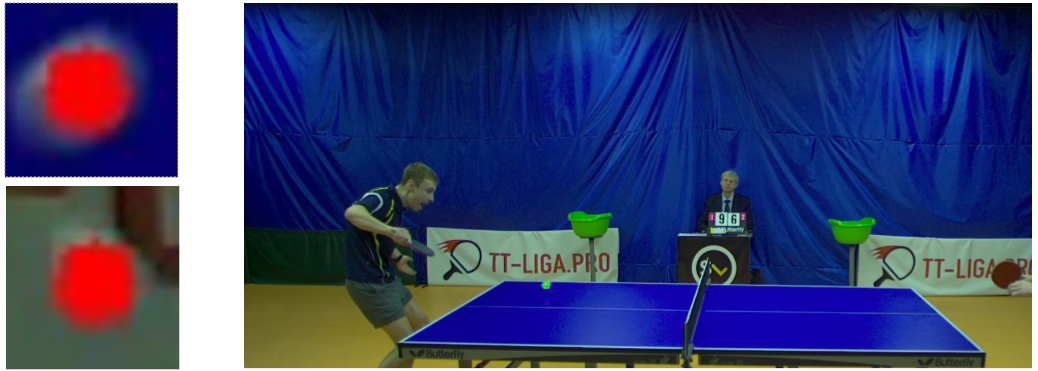
\includegraphics[width=0.8\linewidth]{ball-ping-pong.png}
        \caption{Exemple de adnotări TTNet pentru minge.}
        \label{fig:ping-pong-patch}
    \end{minipage}
\end{figure}

În final am obținut un set de 10.000 de imagini adnotate, fiecare conținând o fereastră de încadrare pentru mingea de tenis de masă, folosindu-le pentru a antrena modelul YOLO.

\subsubsection{Adnotarea paletelor de tenis de masă}

Baza de date TTNet nu conține adnotări pentru palete, așa că vom adapta o metodă similară celei descrise în Secțiunea~\ref{subsec:personal-dataset}. Totuși, modelul GDINO a generat numeroase detecții fals pozitive, cauzate de elemente de fundal, în Figura~\ref{fig:paddle-false-pozitive} putem observa că paleta din decor este detectată drept o paletă reală.

Pentru a gestiona această problemă, vom adapta abordarea de segmentare semantică a obiectelor (Secțiunea \ref{subsec:table-notation}) cu cea de detectare a evenimentelor (Secțiunea \ref{subsec:event-adnotation}), creând o interfață grafică care afișează toate detecțiile inițiale (în fereastre de încadrare roșii) și ne permite să selectăm manual detecțiile corecte (marcate cu fereastre de încadrare verzi), așa cum se poate observa în Figura~\ref{fig:paddle-selected}.

Această soluție semi-automată ne permite adnotarea eficientă a 5.000 de exemple pentru paletele de tenis de masă.


\begin{figure}[H]
    \centering
    \begin{minipage}{\linewidth}
        \centering
        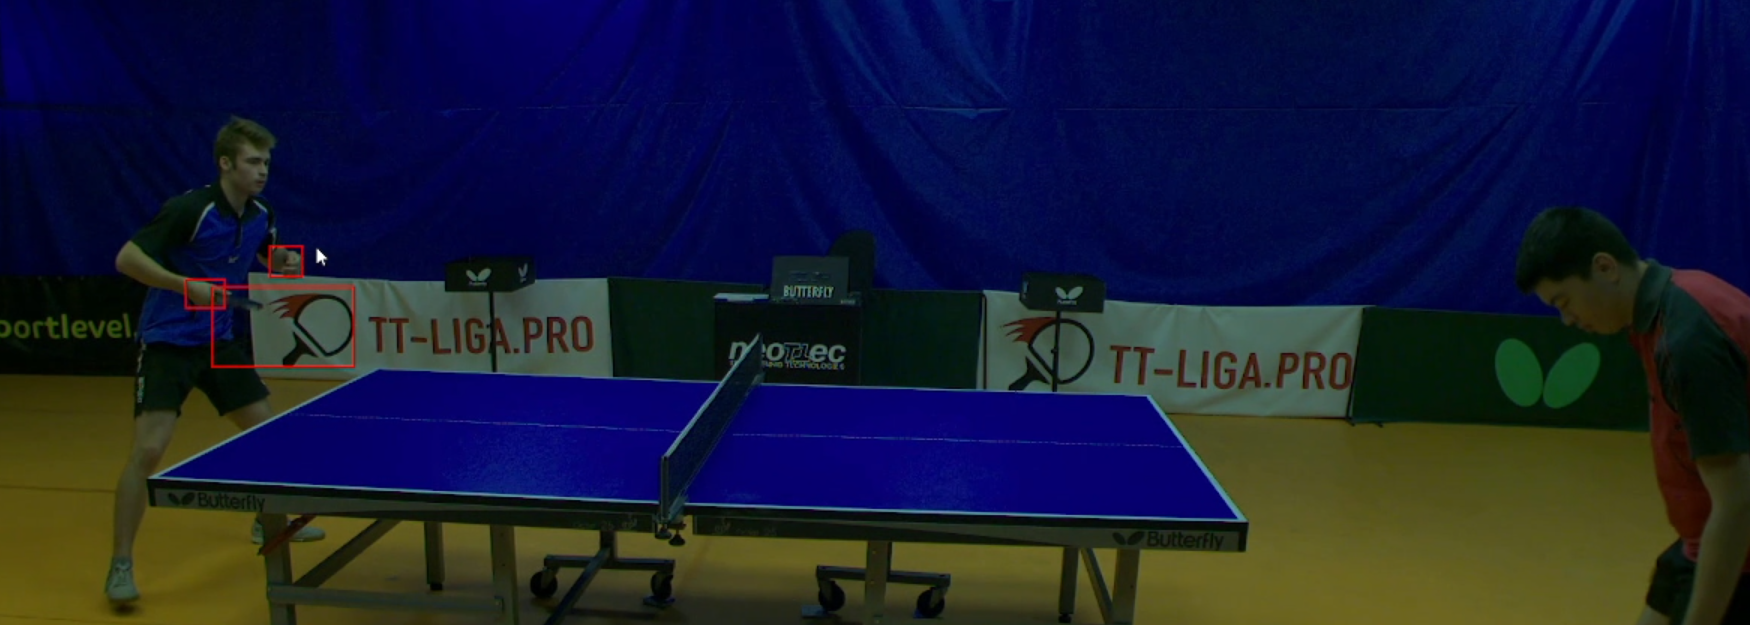
\includegraphics[width=0.8\linewidth]{images/paddle-false-pozitive.png}
        \caption{Exemplu de fals pozitiv generat de GDINO.}
        \label{fig:paddle-false-pozitive}
    \end{minipage}
    \vspace{0.5cm} 
    \begin{minipage}{\linewidth}
        \centering
        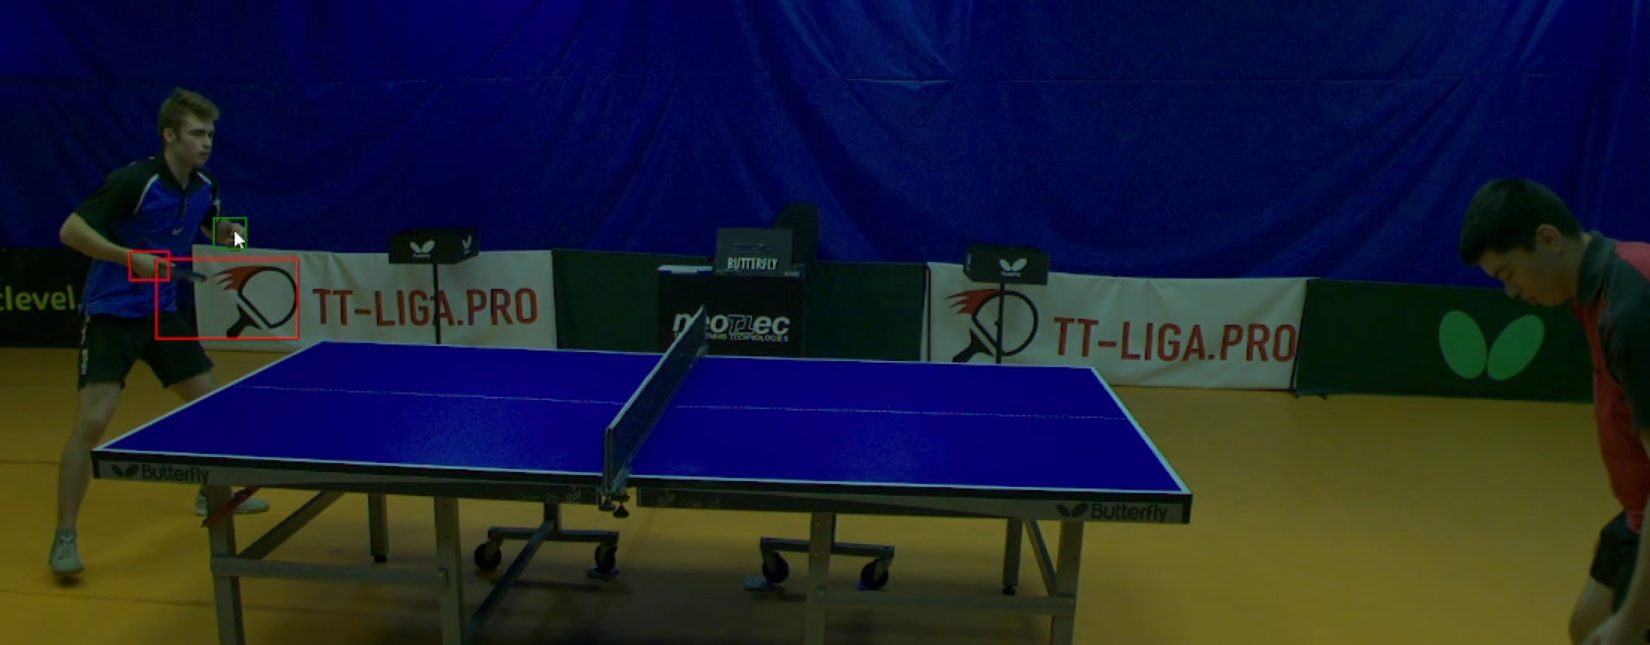
\includegraphics[width=0.8\linewidth]{images/paddle-selected.png}
        \caption{Selecția manuală a adnotărilor corecte.}
        \label{fig:paddle-selected}
    \end{minipage}
\end{figure}

